\documentclass{article}
\usepackage{floatflt,epsfig}
\usepackage[utf8]{inputenc}
\usepackage[T1]{fontenc}
\usepackage{lipsum}
\usepackage{graphicx}
\usepackage{float}
\usepackage{amsmath}
\usepackage[margin=1in]{geometry}
\usepackage{titlesec}
\usepackage{listings}
\usepackage{xcolor}
\usepackage{hyperref}
\usepackage{subfigure}


\hypersetup{
    pdfborder = {0 0 0},
}

\lstdefinelanguage{Java}{
    keywords={abstract,assert,boolean,break,byte,case,catch,char,class,const,continue,default,do,double,else,enum,extends,false,final,finally,float,for,goto,if,implements,import,instanceof,int,interface,long,native,new,null,package,private,protected,public,return,short,static,strictfp,super,switch,synchronized,this,throw,throws,transient,true,try,void,volatile,while},
    morekeywords={[2]System,out},
    morecomment=[l]{//},
    morecomment=[s]{/*}{*/},
    morestring=[b]",
    basicstyle=\small\ttfamily,
    keywordstyle=\color{blue}\bfseries,
    keywordstyle={[2]\color{orange}\bfseries},
    commentstyle=\color{green!70!black},
    stringstyle=\color{red},
    showstringspaces=false,
    tabsize=2,
    breaklines=true,
    breakatwhitespace=true,
    frame=single,
    captionpos=b
}

\titleformat{\section}
{\LARGE\bfseries}{\thesection}{1em}{}

\titleformat{\subsection}
{\Large\bfseries}{\thesection}{1em}{}

\begin{document}

    \pagestyle{empty}

    \begin{titlepage}
        \begin{center}
        {{\Large{\textsc{Alma Mater Studiorum - Università di Bologna}}}}
            \rule[0.1cm]{\textwidth}{0.1px}
            \rule[0.5cm]{\textwidth}{0.6px}\\
            {\large{SCUOLA DI SCIENZE \\ Corso di Laurea in Informatica per il Management}}
        \end{center}

        \vspace{90px}

        \begin{center}
            \LARGE Personal Physical Tracker
        \end{center}

        \vspace{100px}
        \par
        \noindent
        \hfill
        \begin{minipage}[t]{0.4\textwidth}\raggedleft
        {\fontsize{12}{13}{}\
            \fontsize{12}{13}{\\ Canghiari Matteo \\ Matricola 1032059 \\ matteo.canghiari@studio.unibo.it}}

        {\fontsize{12}{13}{}\
            \fontsize{12}{13}{\\ Rocca Claudio \\ Matricola 1020395 \\ claudio.rocca@studio.unibo.it}}
        \end{minipage}

        \vspace*{140px}

        \begin{center}
            \large{Laboratorio di Applicazioni Mobili}\\
            \large{Anno Accademico 2023/2024}
        \end{center}
    \end{titlepage}

    \newpage
    \subsection*{Introduzione}
    \large

    \textbf{Personal Physical Tracker}, è un'applicazione nativa Android che permette di registrare le attività compiute durante la giornata, contraddistinte in \textbf{camminata}, \textbf{spostamenti in macchina} e \textbf{attività sedentarie}.
    L'applicazione si avvale di differenti funzionalità, dalla registrazione delle attività compiute sino alla visualizzazione dei dati di altri utenti presenti sull'applicativo. Tutte le funzionalità sviluppate saranno successivamente approfondite nella sezione \textbf{Feature}, tuttavia è possibile anticipare ciò che contraddistingue il sistema software ideato. \vspace*{7pt}\\
    Ad un primo avvio l'utente visualizza la schermata per la registrazione in cui può effettuare il \textit{Sign In} in caso di un nuovo utente, o il \textit{Login} in caso di utente già registrato. Proseguendo, viene mostrata la schermata Home dell'app, composta da una \textit{Navigation Bottom Bar}, che garantisce l'accesso diretto alle funzionalità sviluppate. \\
    Tramite la Navigation Bar l'utente ha la possibilità di \textbf{registrare} nuove attività, \textbf{visualizzare} il proprio storico, osservare le proprie \textbf{aree geografiche di interesse}, visualizzare i \textbf{grafici} relativi alle proprie attività registrate ed, infine, condividere e visualizzare le attività condivise da altri utenti nella sezione \textbf{amici}. \vspace*{7pt}\\
    Di seguito vengono brevemente descritte alcune scelte implementative e strumenti utilizzati durante lo sviluppo dell'app: per il versionamento del codice è stato utilizzato \textbf{Git}, con repository accessibile su \textbf{GitHub}, mentre per lo sviluppo dell'applicativo è stato utilizzato il linguaggio di programmazione \textbf{Kotlin}, per la realizzazione di un'applicazione \textbf{nativa Android}. Il progetto si compone di tre punti cardine per il corretto funzionamento, suddivisi come segue:
    \begin{itemize}
        \renewcommand{\labelitemi}{-}
        \item Design pattern architetturale \textbf{MVVM}, utilizzato per separare i componenti \textbf{Model}, ovvero il \textit{contenitore di dati}, e la sezione \textit{attiva}, la \textbf{View} mostrata direttamente all'utente. In questo modo si garantisce la separazione tra i componenti, riducendo l'accoppiamento e le \textit{dipendenze funzionali}, che potrebbero causare danni ai componenti dell'applicazione anche in seguito a piccole modifiche
        \item \textbf{Room}, utilizzato per garantire la persistenza dei dati all'interno di un \textit{Database Relazionale}
        \item \textbf{Amazon S3}, utilizzato per salvare in cloud i dati degli utenti attraverso un \textit{database dump}, consentendo la condivisione dei dati salvati sul \textit{database locale} e permettendo di visualizzare i dati condivisi dagli amici
    \end{itemize}

    \newpage
    \subsection*{Feature}
    \textit{Registrazione} \vspace*{7pt}\\
    All'avvio dell'app è richiesta la registrazione delle credenziali, suddivise in \textit{username} e \textit{password}. E' necessario registrarsi con un username non ancora presente, per garantire l' univocità dei dati. Una volta registrato, all'utente sarà richiesto di concedere tutti i permessi necessari per il funzionamento dell'applicazione. L'applicazione utilizza la connessione internet per controllare se un altro utente si è già registrato in passato con lo stesso username, è pertanto necessario avere una connessione dati per registrarsi all'app.\\
    Tra i permessi richiesti sono presenti:
    \begin{itemize}
        \renewcommand{\labelitemi}{-}
        \item \textbf{Access fine location}, autorizzazione di accesso alla posizione corrente del dispositivo, necessaria per monitorare le aree geografiche varcate
        \item \textbf{Access background location}, permesso necessario per accedere alla posizione del dispositivo anche quando l'applicazione è in secondo piano
        \item \textbf{Post notifications}, consente di inviare notifiche al dispositivo
    \end{itemize}
    Qualora siano negati i permessi richiesti non sarà consentito l'utilizzo dell'applicazione; ad un nuovo avvio è mostrato un \textit{Alert Dialog} in cui è richiesto all'utente di abilitare le autorizzazioni necessarie tramite \textit{Impostazioni}. \vspace*{7pt}\\
    \begin{center}
        \begin{figure}[H]
            \centering
            \subfigure[Sign In fragment]{
                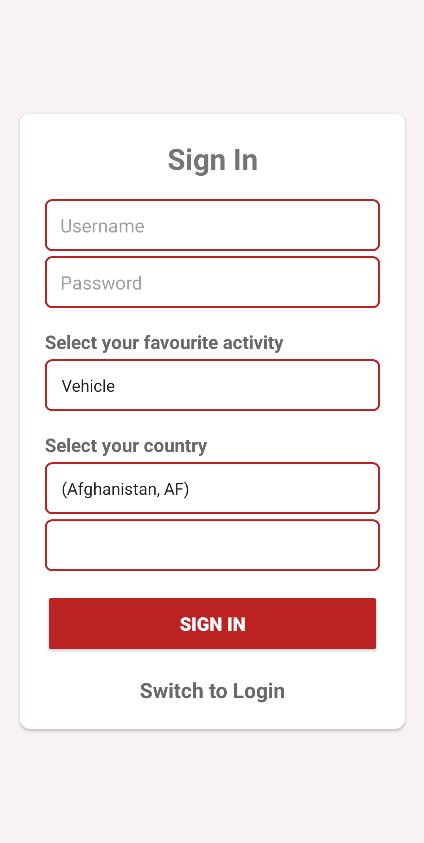
\includegraphics[width=0.35\textwidth]{img1.png}
            }
            \subfigure[Login fragment]{
                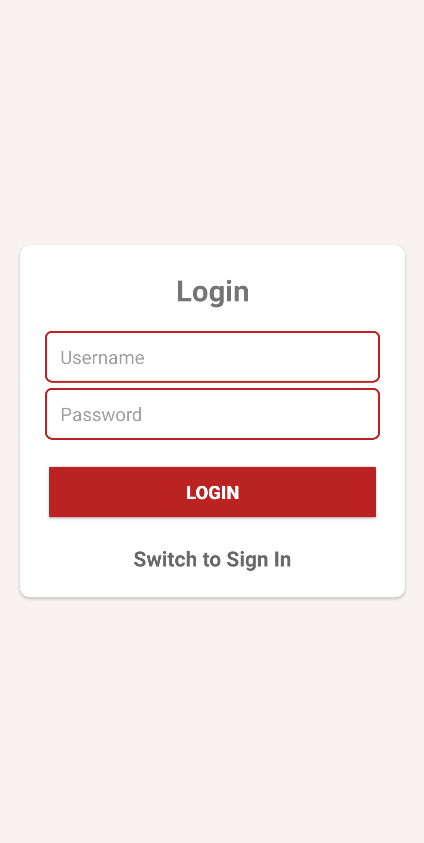
\includegraphics[width=0.35\textwidth]{img2.png}
            }
        \end{figure}
    \end{center}
    \textit{Registrazione attività} \vspace*{7pt}\\
    Proseguendo, successivamente all'autenticazione, è possibile registrare le attività compiute durante la giornata cliccando sul \textit{floating button} presente nella schermata \textbf{Home}, \textbf{Calendario} e \textbf{Grafici}. L'utente può registrare le seguenti attività:
    \begin{itemize}
        \renewcommand{\labelitemi}{-}
        \item \textbf{Attività sedentaria}, in cui è definito il tempo trascorso
        \item \textbf{Camminata}, in cui sono memorizzati i passi fatti e il dislivello percorso durante la registrazione
        \item \textbf{Spostamenti in macchina}, durante i quali viene registrata la distanza percorsa
    \end{itemize}
    Tutti i dati relativi alle attività dell'utente vengono salvati in un database locale e rielaborati per consentirne la visualizzazione grafica. Per consentire ciò è necessario che l'utente, abbia in precedenza autorizzato il permesso \textbf{Activity recognition}. Quest'ultimo garantisce di identificare propriamente l'avvio oppure l'interruzione di un'attività. \vspace*{7pt}\\
    \textit{Nota bene}: nel progetto proposto la funzionalità legata al \textbf{detect} dell'attività in corso non consiste in un'\textbf{operazione in background}.
    \begin{center}
        \begin{figure}[H]
            \centering
            \subfigure[Registrazione nuove attività]{
                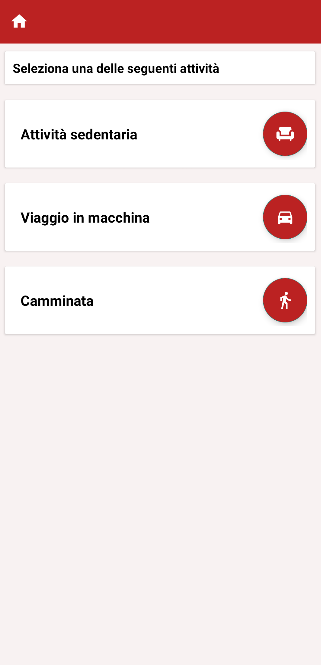
\includegraphics[width=0.35\textwidth]{img3.png}
            }
            \subfigure[Avvio/Interruzione registrazione attività]{
                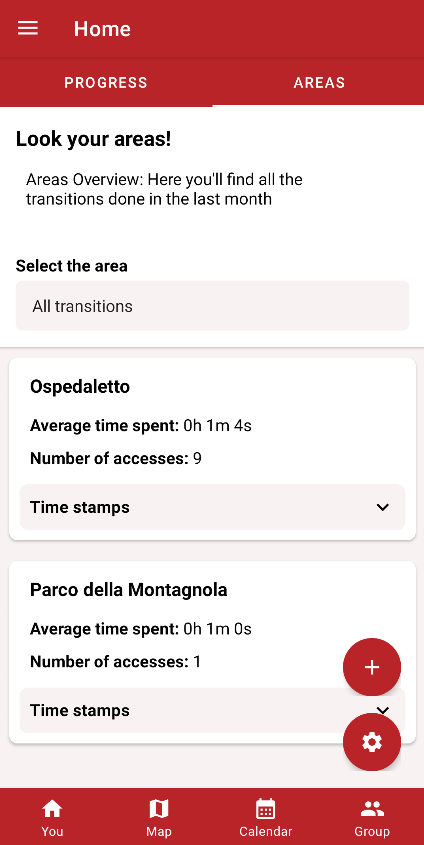
\includegraphics[width=0.35\textwidth]{img4.png}
            }
        \end{figure}
    \end{center}
    \textit{Calendario} \vspace*{7pt}\\
    L'utente può visualizzare nel \textbf{calendario} tutte le attività registrate. Cliccando su una cella che compone il \textit{calendario}, è possibile visualizzare le attività compiute nella giornata selezionata e le relative informazioni, oltre ad un \textit{grafico a torta} che riporta il tempo speso per i vari tipi di attività durante l'arco temporale prestabilito, specificando la porzione di tempo di cui non si hanno dati a disposizione.
    \begin{center}
        \begin{figure}[H]
            \centering
            \subfigure[Calendario]{
                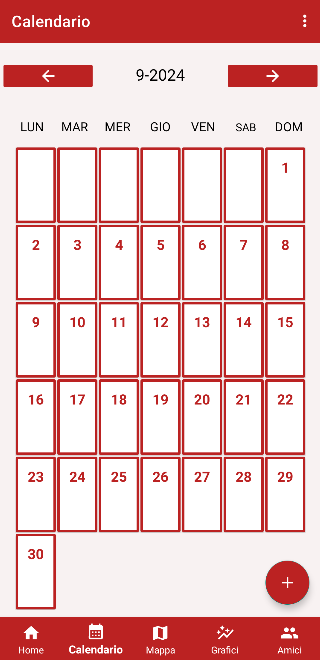
\includegraphics[width=0.35\textwidth]{img5.png}
            }
            \subfigure[Visualizzazione attività]{
                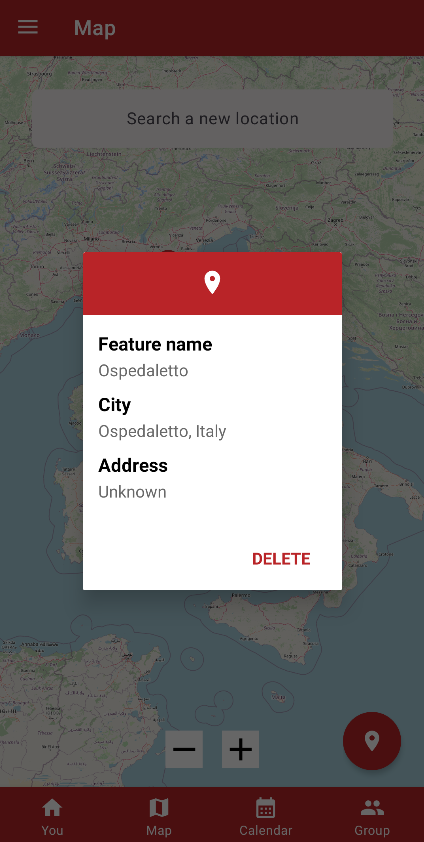
\includegraphics[width=0.35\textwidth]{img6.png}
            }
        \end{figure}
    \end{center}
    \textit{Grafici} \vspace*{7pt}\\
    La feature \textit{grafici} permette di visualizzare in maniera intuitiva i dati registrati dall'applicazione nel mese selezionato. La \textit{View} è composta da tre grafici, cosi suddivisi:
    \begin{itemize}
        \renewcommand{\labelitemi}{-}
        \item \textbf{Grafico a barre}, contenente i \textbf{passi fatti} dall'utente per ogni giorno che componga il mese registrati durante attività di \textit{camminata}
        \item \textbf{Grafico a barre}, utilizzato per visualizzare la \textbf{distanza percorsa} dall'utente ogni giorno durante le attività di \textit{spostamento con veicolo}
        \item \textbf{Grafico a torta}, che riporta in percentuale la suddivisione per \textbf{tipo di attività} registrate dall'utente
    \end{itemize}
    \textit{Mappa} \vspace*{7pt}\\
    La \textit{View} contiene una \textbf{mappa} all'interno di un \textit{FragmentContainerView}. L'utente può inserire, visualizzare ed eliminare le \textit{aree geografiche di interesse}, registrate all'interno del \textit{database locale}. Una zona di interesse è l'area compresa nel raggio di [150m, 250m] rispetto alle coordinate geografiche selezionate, varcata la soglia di una di esse l'utente riceve una notifica. \vspace*{7pt}\\
    \textit{Nota bene}: il funzionamento della feature è garantito solamente in presenza di una \textbf{connessione dati stabile}.
    \begin{center}
        \begin{figure}[H]
            \centering
            \subfigure[Mappa]{
                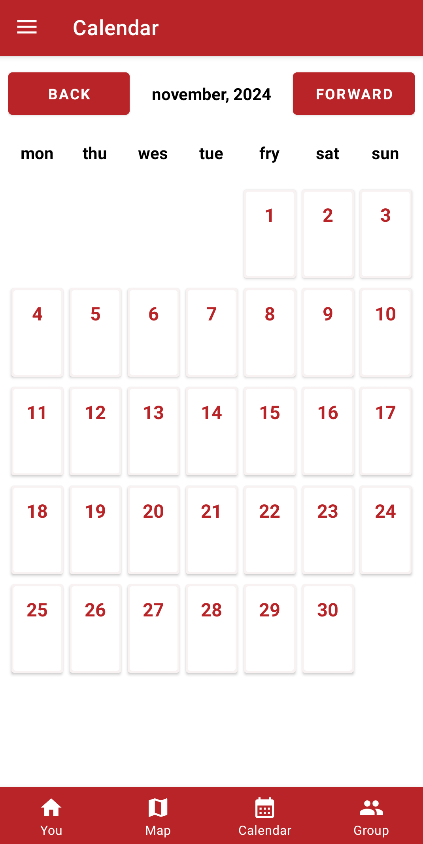
\includegraphics[width=0.35\textwidth]{img7.png}
            }
            \subfigure[Dialog dei marker sulla mappa]{
                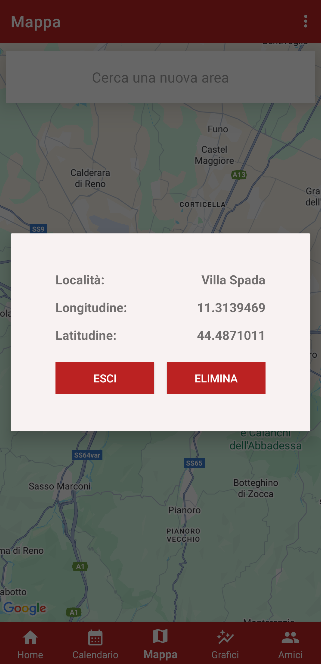
\includegraphics[width=0.35\textwidth]{img8.png}
            }
        \end{figure}
    \end{center}
    \textit{Amici} \\
    Tramite l'applicativo è possibile condividere le proprie attività con altri \textbf{utenti} utilizzatori e visualizzare le stesse da loro compiute. Un utente può cercare lo \textit{username} di un amico per poi aggiungerlo alle proprie \textbf{amicizie} e visualizzare le attività da esso memorizzate.
    Precedentemente alla condivisione dei dati, viene mostrato un \textit{Alert Dialog} che richiede l'autorizzazione per il salvataggio dei dati in cloud, se il permesso dovesse essere negato sarà comunque possibile visualizzare i dati degli amici.
    Inoltre, l'utente può sincronizzare i dati salvati in \textit{cloud} in qualsiasi momento, cliccando sul \textit{floating button} presente nella schermata. \vspace*{7pt}\\
    \textit{Nota bene}: il funzionamento della feature è garantito solamente in presenza di una \textbf{connessione dati stabile}.
    \begin{figure}[H]
        \centering
        \subfigure[Amici fragment]{
            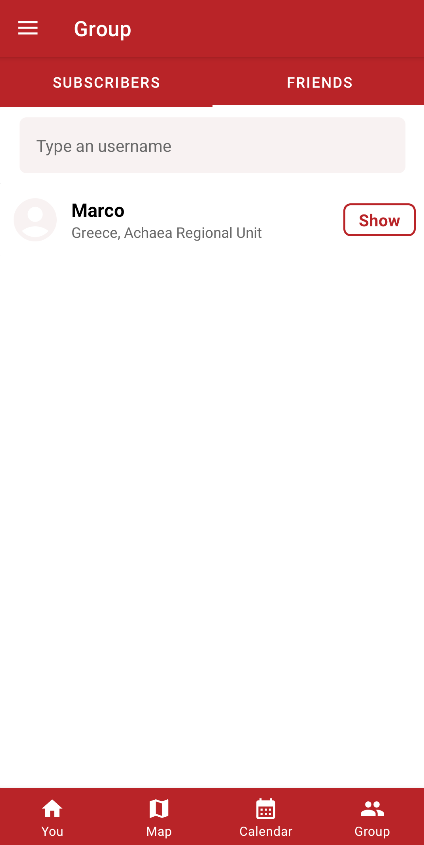
\includegraphics[width=0.35\textwidth]{img9.png}
        }
        \subfigure[Visualizzazione dati amico]{
            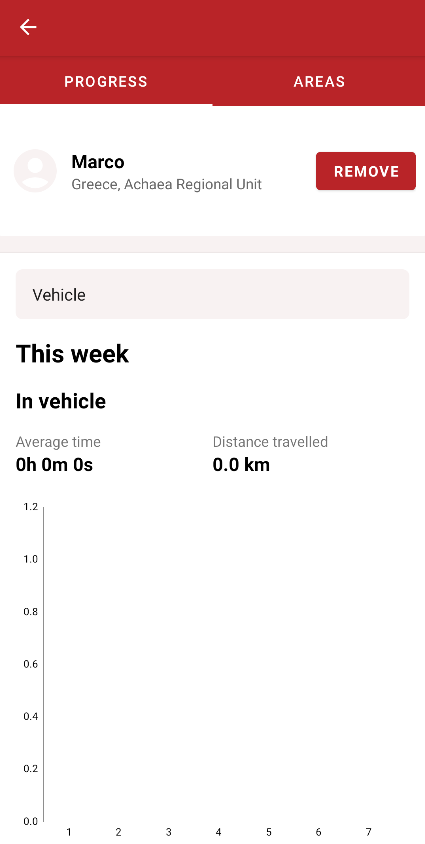
\includegraphics[width=0.35\textwidth]{img10.png}
        }
    \end{figure}

    \newpage
    \subsection*{Scelte implementative}
    \subsubsection*{RecyclerView}
    Questo tipo di view è stata utilizzata per la rappresentazione delle attività dell'utente, essa è infatti ottimizzata per gestire grandi quantità di dati pur garantendo buone prestazioni nella velocità di caricamento. La Recycler View ricicla infatti i dati al di fuori della view che per consentire di ridurre la memoria utilizzata. \vspace*{7pt}\\
    Negli screenshot riportati, la RecyclerView è stata utilizzata nelle schermate Home, Calendario e Amici, riutilizzando il codice per caricare i dati all'interno delle card. In diverse occasioni sono state implementate funzionalità direttamente nei singoli ViewHolder, operazione resa possibile grazie al binding dei parametri, semplificato dall'uso degli Adapter. Questo approccio permette una gestione più efficiente e flessibile dei dati nelle varie sezioni dell'app.
    \subsubsection*{ViewModel}
    Come già accennato nell'introduzione, uno dei punti cardine su cui si basa il progetto è il design pattern architetturale \textbf{Model-View-ViewModel}. \\
    Questo approccio separa la \textit{View}, definita \textbf{entità attiva}, poichè al suo interno è sviluppata la \textit{business logic}, e il Model, \textbf{entità passiva}, contenitore statico di dati. \vspace*{7pt}\\
    Il \textbf{ViewModel} è incaricato di mantenere aggiornate le strutture dati che acquisiscono informazioni dal \textit{Model}. Ciò avviene per garantire che tutti i soggetti il cui comportamento può variare al cambiamento dei dati contenuti nel \textit{Model}, possano essere notificati dinnanzi ad una qualsiasi modifica. Questo comportamento è stato ottenuto attraverso l'impiego di \textbf{LiveData}, i quali si basano sul concetto di \textit{Observables}.
    \begin{lstlisting}[language = JAVA]
class NetworkViewModel: ViewModel() {
    private val _currentNetwork = MutableLiveData<Boolean>()
    val currentNetwork: LiveData<Boolean> get() = _currentNetwork

    init {
        _currentNetwork.value = MyNetwork.isConnected
    }

    fun setNetwork(enabled: Boolean) {
        viewModelScope.launch(Dispatchers.Main) {
            if (_currentNetwork.value != enabled) {
                _currentNetwork.value = enabled
            }
        }
    }
}
    \end{lstlisting}
    La sezione di codice riportata definisce il metodo utilizzato per mantenere aggiornati i \textit{Fragment} interessati allo stato corrente della \textit{connessione}. All'interno delle classi è implementata una funzione incaricata di osservare cambiamenti del \textit{LiveData currentNetwork}, abilitando oppure disabilitando le funzionalità che richiedono una connessione.
    \subsubsection*{Room}
    Per garantire la persistenza dei dati è stata utilizzata la libreria \textbf{Room}. \textit{Room} permette di gestire con semplicità un \textit{Database Relazionale}, consentendo la gestione automatica di aggiornamento del database, causato per esempio dall'introduzione di una nuova tabella o dalle modifiche apportate alla struttura di una esistente. \vspace*{7pt}\\
    L'implementazione di \textit{Room} è piuttosto intuitiva. Dichiarata un'instanza del database, è necessario creare le differenti tabelle che caratterizzano il \textit{Modello E-R} dedotto e i loro \textbf{DAO}, ossia classi in cui sono definite le principali interazioni possibili con il database.
    \begin{lstlisting}[language = JAVA]
@Database(
    entities = [UserEntity::class, UserStillActivityEntity::class, UserVehicleActivityEntity::class, UserWalkActivityEntity::class, GeofenceAreaEntry::class, FriendEntity::class],
    version = ROOM_DATABASE_VERSION
)
abstract class BrockDB: RoomDatabase() {
    abstract fun UserDao(): UserDao
    abstract fun UserStillActivityDao(): UserStillActivityDao
    abstract fun UserVehicleActivityDao(): UserVehicleActivityDao
    abstract fun UserWalkActivityDao(): UserWalkActivityDao
    abstract fun GeofenceAreaDao(): GeofenceAreaDao
    abstract fun FriendDao(): FriendDao


    companion object {
        @Volatile
        var INSTANCE: BrockDB? = null

        @Synchronized
        fun getInstance(context: Context): BrockDB {
            if (INSTANCE == null) {
                INSTANCE = Room.databaseBuilder(
                    context,
                    BrockDB::class.java,
                    "brock.db"
                ).fallbackToDestructiveMigration()
                    .build()
            }
            return INSTANCE as BrockDB
        }
    }
}
    \end{lstlisting}
    Come è possibile osservare dallo snippet di codice proposto, il database è composto da sei \textit{tabelle}, ad ognuna delle quali è associato il proprio \textit{DAO}.
    Inoltre, seguendo il \textit{design pattern Singleton}, è realizzata una sola istanza del \textit{database}, per garantire che tutte le operazioni di lettura e scrittura siano sincronizzate e che facciano riferimento agli stessi dati.

    \subsubsection*{Background operations}
    Le \textbf{operazioni in background} sviluppate all'interno del progetto si suddividono in due sezioni, cosi descritte:
    \begin{itemize}
        \renewcommand{\labelitemi}{-}
        \item \textbf{Geofencing}, recinti virtuali utilizzati per contrassegnare località di interesse. A partire dalle coordinate geografiche scelte dall'utente viene registrata un'area circolare, rispetto ad un raggio prestabilito. Qualora l'utente dovesse varcare la soglia di una di queste are, l'applicativo invia una notifica al dispositivo
        \item \textbf{Connectivity}, utilizzato per accertarsi della presenza di una \textit{connessione ad Internet} stabile, abilitando oppure disabilitando determinate funzionalità richiedenti una connessione dati. Tale approccio è utilizzato soprattutto per ovviare a comportamenti indesiderati dell'applicazione
    \end{itemize}
    \begin{center}
        \begin{figure}[H]
            \centering
            \subfigure[Notifica proveniente da Geofencing]{
                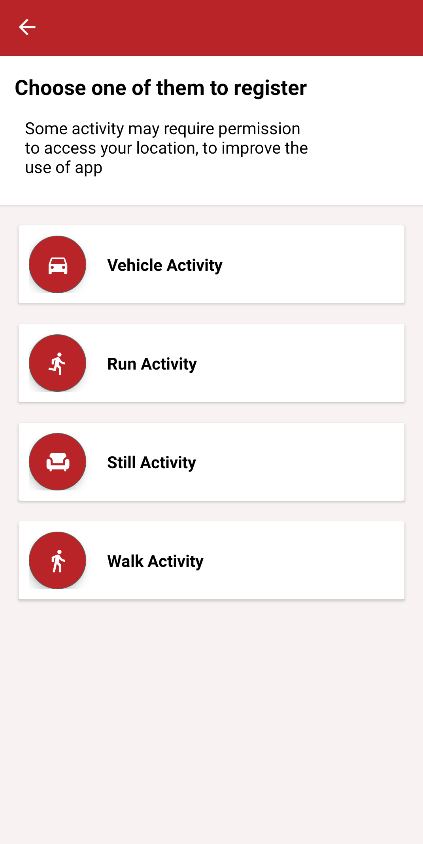
\includegraphics[width=0.35\textwidth]{img11.png}
            }
            \subfigure[Notifica proveniente da Connectivity]{
                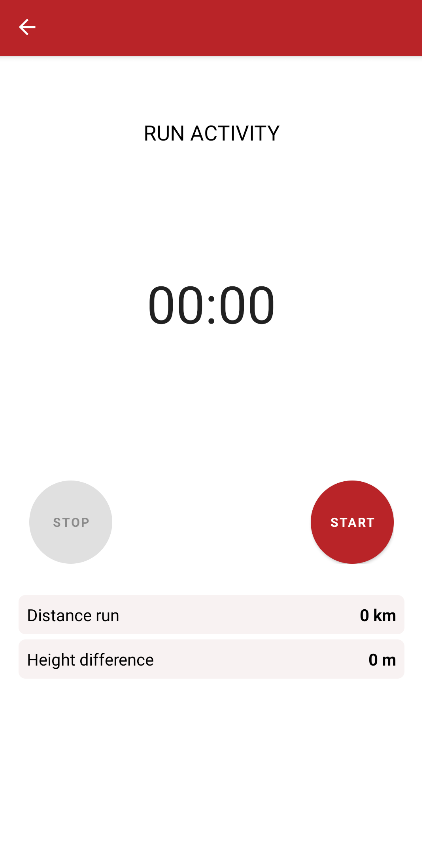
\includegraphics[width=0.35\textwidth]{img12.png}
            }
        \end{figure}
    \end{center}
    \textit{Geofencing} \\
    Come già accennato, l'operazione in questione controlla attivamente qualora l'utente varchi i confini di un'area di interesse. A questo scopo, è stato implementato un \textbf{Broadcast Receiver} capace di intercettare intenti lanciati dai componenti che registrano la posizione dell'utente. Un \textbf{Worker} viene poi incaricato di notificare il dispositivo dell'utente.\vspace*{7pt}\\
    \textit{Connectivity} \\
    Contrariamente a quanto fatto per il Geofencing, in questo caso è stato utilizzato un \textbf{Service}. Nuovamente, è stato implementato un \textbf{Broadcast Receiver} affinchè possano essere gestiti cambiamenti della connessione. Una volta ricevuto l'intento viene richiamato il \textit{Service}, in cui è controllato lo stato della connessione: a seconda della disponibilità della connessione vengono abilitate o disabilitate le feature che richiedono l'accesso ad Internet.\\
    Infine, è avviato un \textbf{Worker} incaricato di notificare l'utente in caso di cambiamenti significativi della connessione. \vspace*{7pt}\\
    Tuttavia, è bene affermare che il \textit{Service} descritto è utilizzato anche per modificare la dimensione dell'aree di interesse. In base alla tipologia di \textit{connessione ad Internet} presente, il servizio provvederà a modificare il raggio delle \textit{aree di interesse}, in ottica di risparmio energetico e per garantire maggiore accuratezza anche in caso di connessione scarsa.
    \subsubsection*{AWS Simple Storage Service}
    Per consentire agli utenti di condividere i propri dati è stato utilizzato \textit{AWS Simple Storage Service}, la scelta è ricaduta su esso per le conoscenze pregresse del gruppo e per la facile integrazione fornita dalla AWS SDK in Kotlin.\\
    Al momento della condivisione dei dati dell'utente viene effettuato un dump del database in formato JSON: i dati vengono strutturati in questo formato tramite la popolare libreria Gson, per poi essere salvati su un file che viene caricato su un bucket tramite una richiesta formulata da un AwsS3Client come nel seguente codice:\\
    \begin{lstlisting}[language=Java]
    fun uploadUserData() {
        viewModelScope.launch(Dispatchers.Default) {
            val walkActivities = db.UserWalkActivityDao().getWalkActivitiesByUserId(User.id)
            val vehicleActivities = db.UserVehicleActivityDao().getVehicleActivitiesByUserId(User.id)
            val stillActivities = db.UserStillActivityDao().getStillActivitiesByUserId(User.id)

            val userData = mapOf(
                "username" to User.username,
                "walkActivities" to walkActivities,
                "vehicleActivities" to vehicleActivities,
                "stillActivities" to stillActivities
            )

            val gson = Gson()
            val json = gson.toJson(userData)

            val file = File(context.filesDir, "user_data.json")
            file.writeText(json)

            withContext(Dispatchers.IO) {
                try {
                    val request = PutObjectRequest(BUCKET_NAME, "user/${User.username}.json", file)
                    s3Client.putObject(request)
                } catch (e: Exception) {
                    Log.e("S3Upload", "Failed to upload user data", e)
                }
            }

        }
    }

    \end{lstlisting}
    Per cercare un amico l'utente digita lo username della persona desiderata nella barra di ricerca, viene dunque effettuata una richiesta di \textit{getObject} al bucket, che restituisce i dati di tutti gli utenti che hanno come prefisso dello username la stringa inserita dall'utente nella barra di ricerca.

    \subsection*{Possibili sviluppi futuri}
    In un ulteriore sviluppo dell'app sarebbe possibile migliorare i seguenti aspetti:
    \begin{itemize}
        \renewcommand{\labelitemi}{-}
        \item Maggiore sicurezza nella condivisione dei dati in cloud, per garantire l'accesso solo agli utenti autorizzati.
        \item Miglioramento interfaccia ed esperienza utente, per garantire un facile accesso a tutte le funzionalit
        \item Aumento dei servizi in background, come la registrazione automatica delle attività, per eliminare la necessità dell'avvio e dell'interruzione di una attività da parte dell'utente.
        \item Miglioramento gestione batteria, con riduzione delle prestazioni dell'app in caso di batteria scarica
        \item Aggiunta della possibilità di eliminare amici
    \end{itemize}

\end{document}